% what does it mean? Interpret the patterns observed within the data. Link back to a broader discussion.

Shipping is a major user of the ocean, but little is known about its distribution and effects. Here I built the first validated and global models of ship movement, to better enable us to manage the ocean effectively. The shipping companies acknowledge the importance of managing the ocean holistically, but lack the scientific knowledge and tools to do so effectively. By incorporating ecological information alongside logistical efficiencies, it should be possible to improve the system robustness.

Marine protected areas (MPAs) have been shown to be effective~\citep{halpern2002marine}, but the multidimensional nature of ocean use is pointing toward dynamic MPAs, which may rely on providing users, such as ship operators, with real-time information about the state of the environment. Marine spatial planning is proving a promising avenue for brining stakeholders together~\citep{merrifield2012marinemap}. This new form of planning has greater data requirements, which in the ocean can be simplified down to three major areas of use: fisheries management, transportation management, and energy management (Figure \ref{fig:framing}). Transportation in the ocean is the least studied of the three, and here we have shown how volunteered geographic information methods, along with volunteered observations, can provide us a way to tackle the data-poor problem.

% XXX FORMAT THIS AROUND THE TALK SLIDES

% XXX REMOVE THIS? Don't really need it, was really just filler till I had my act together. Explain, IN WORDS, why this matters and integrate those changes into the body of the thesis.
%\begin{figure}[h!]
%  \centering
%    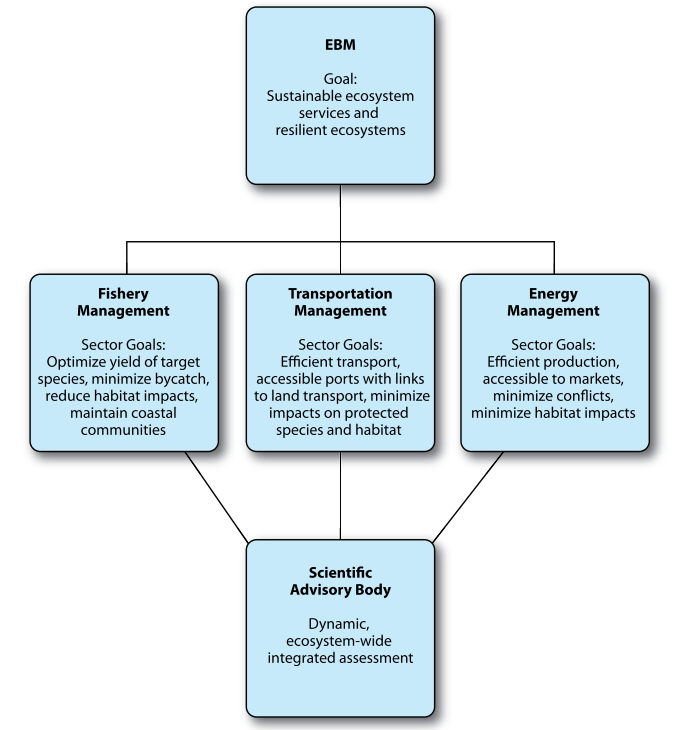
\includegraphics[width=90mm]{figures/lubechenco-diagram.png}
%  \caption[Framing Ecosystem-based management goals]{Framing ecosystem-based management goals, as in \cite{Lubchenco2010}; original from \citep{McLeod2009}}
%  \label{fig:framing}
%\end{figure}
% XXX INCLUDE THE GOALS IN TEXT, fisheries management, transportation, energy production.



% - shipping has big economic benefit, but costs are externalized

% - there are good actors in shipping who want to do the right thing, but don't have the tools to do it [cites, +Maersk lady]

% - only scientific community can do this

% - can only do msp by bringing stakeholders together

% - VGI methods provide good way of handling messy data as we try to move it toward 'reality'

% - coupling these approaches with real-time efforts has potential to shift dynamic.
